\documentclass[fr]{../../../eplsummary}

\hypertitle{Stratégie d'entreprise}{6}{ECGE}{1315}
{Florian Thuin}
{Vincent Meurisse}

\section{Introduction à la stratégie}

\subsection{Définitions}

La \textbf{stratégie} est l'orientation à \textit{long terme} d'une
organisation. Elle est définie par des décisions \textbf{délibérées} et
\textbf{rationnelles}, \textbf{émergentes} et
\textbf{incrémentales}.\newline

Typiquement, un stratégie consiste à développer un avantage
concurrentiel durable, une coopération avec d'autres organisations  ou
une imitation de celles-ci.\newline

\textbf{DAS} : Domaine d'activité stratégique. Dans une entreprise de
grande taille, on divise l'entreprise en parties pour lesquelles on
appliquera une stratégie différentiée (ex: Virgin Airlines et Virgin
Music n'ont pas la même stratégie).\newline

\textbf{Degré de concentration} : plus le nombre d'entreprises à exercer
une activité est faible, plus le degré de concentration est élevé.
Autrement dit, un degré de concentration élevé entraîne un pouvoir de
négociation fort des personnes qui exercent ces activités.\newline

\textbf{Intégration vers l'amont} : fusion ou rachat d'un
fournisseur\newline

\textbf{Intégration vers l'aval} : fusion ou rachat d'un client\newline

\textbf{Coût de transfert} : prix à payer pour passer d'un collaborateur
à un autre (par ex: changer de fournisseur). Un prix faible entraîne une
intensité concurrentielle plus forte, on peut augmenter le prix en liant
les clients par des contrats avec clause de résiliation.\newline

\textbf{Facteur clé de succès (FCS)} : éléments stratégiques qu'une
organisation doit maîtriser afin de surpasser la concurrence.
Généralement lié à la création de valeur pour le client, ils permettent
de contrecarrer les forces (modèle de Porter) de la concurrence.
\newline

\textbf{La chaîne de valeur} : les différentes étapes permettant à une
organisation d'obtenir une offre valorisée par ses clients. \newline

\textbf{La filière} : succession de liens interorganisationnels et
d'activités nécessaires à la création d'une offre.\newline 

\subsection{Horizons}

\paragraph{Management de l'analyse} L'horizon 1 consiste à étendre et à
défendre l'activité principale.

\paragraph{Management de l'exploration} L'horizon 2 consiste à
construire des activités émergentes.

\paragraph{Management de l'imagination} L'horizon 3 consiste à créer des
options viables de développement.

\subsection{Caractéristiques}

Une bonne stratégie a pour objectifs de satisfaire toutes les parties
prenantes en obtenant et développant un \textbf{avantage concurrentiel
durable}. Elle consiste à allouer des ressources qui engage
l'organisation dans le long terme créant ainsi un \textbf{périmètre d'activité}.

Elle doit :
\begin{enumerate}
    \item entraîner un \color{red} surcroit de valeur \color{black} pour les clients
    \item définir un \color{red} modèle économique difficilement
        imitable \color{black}
\end{enumerate}

\subsection{Le modèle VIP}

\begin{description}
    \item[V]aleur : définir le modèle de création de valeur pour les
        parties prenantes (\textit{value proposition}).
    \item[I]mitation : la value proposition doit être difficilement
        imitable pour assurer l'avantage concurrentiel \textbf{durable}.
    \item[P]érimètre : définir un périmètre (que faire ou non : marchés
        et activités)
\end{description}

\subsubsection{Exemple Ikea}

\begin{description}
    \item[Valeur] : bas prix et tout au même endroit (économie
        d'échelle), stockage facile, repartir directement avec ce qu'on
        achète, très large gamme de produits, services annexes
    \item[Imitation] : impossible de faire la même chose à grande
        échelle ou à prix inférieur, designers exclusifs, adaptations
        locales
    \item[Périmètre] : activité : limité au mobilier d'intérieur et à la
        présentation ; marché : international
\end{description}

\subsection{Les niveaux de stratégie}

\begin{enumerate}
    \item Stratégie d'entreprise (CORPORATE) : stratégie globale de
        l'entreprise
    \item Stratégie par domaine d'activité (BUSINESS) : une entreprise
        de grande taille est divisée en DAS qui auront chacun une
        stratégie différentiée basée sur la stratégie de l'entreprise.
    \item Décisions opérationnelles : déploiement  de la stratégie
        décidée par des décisions précises
\end{enumerate}

\subsection{Formuler une stratégie}

Une stratégie doit définir les buts fondamentaux d'une organisation,
autrement dit :

\begin{description}
    \item[La mission] : expression du but général de l'organisation
    \item[La vision] : état futur souhaité pour l'organisation
    \item[Les objectifs] : précis en horizon temporel et quantitatifs
    \item[Le périmètre d'activité] : notre métier et nos clients
    \item[L'avantage concurrentiel] : ce qui fait qu'on ajoute plus de
        valeur au produit qu'un concurrent (selon le client)
\end{description}

\subsubsection{Objectifs SMART}

Tout objectif défini par une entreprise doit être SMART, autrement dit :

\begin{description}
    \item[S]pécifique
    \item[M]esurable
    \item[A]tteignable
    \item[R]éaliste
    \item[T]emporel
\end{description}

\subsection{Etablir une stratégie}

Une stratégie se définit par trois composantes interdépendantes :

\begin{description}
    \item[Le diagnostic stratégique] : définit le contexte de l'organisation
    (culturel, concurrentiel, économique,\ldots)
    \item[Le déploiement stratégique] : définit les processus utilisés
    \item[Les choix stratégiques] : définit le contenu de la stratégie
\end{description}

\section{Le diagnostic stratégique}

Un diagnostic stratégique consiste à mettre en lumière le contexte dans
lequel l'entreprise évolue pour mieux comprendre comment développer une
stratégie viable à long terme.

\subsection{Analyse PESTEL}

Le modèle PESTEL met en avant les \textit{variables pivots} de
l'évolution du macroenvironnement (une seule analyse est nécessaire pour
toute l'entreprise).

\begin{description}
    \item[P]olitiques : rôle des pouvoirs publics
    \item[E]conomiques : facteurs macroéconomiques (taux d'intérêt, PIB)
    \item[S]ociologiques : évolutions culturelles/démographiques
    \item[T]echnologiques : impact des innovations
    \item[E]nvironnementales : préoccupations écologiques
    \item[L]égales : contraintes juridiques
\end{description}

On liste tout ce qui rend en compte (positivement et négativement) et
ensuite on définit des facteurs majeurs (variables pivots, \textit{key
drivers}) ce qui va nous permettre de définir 2 ou 4 scénarios possibles
pour le secteur d'activité.

\subsection{Analyse des 5+1 forces (Porter)}

Le modèle de Porter permet d'évaluer l'attractivité d'une industrie en
termes d'\textbf{intensité concurrentielle} (une analyse est nécessaire
par DAS). \newline

Plus l'intensité de ces forces est élevée, plus le secteur est
inattractif :

\begin{itemize}
    \item[1.] Les \color{green!80!black} entrants \color{black} potentiels
    \item[2.] Le pouvoir de négociation des
        \color{green!80!black}acheteurs\color{black}
    \item[3.] Le pouvoir de négociation des
        \color{green!80!black}fournisseurs\color{black}
    \item[4.] La menace des \color{green!80!black}produits de
        substitution\color{black}
    \item[5.] \textbf{L'intensité concurrentielle}
    \item[+1] Le rôle des \color{green!80!black}pouvoirs publics
\end{itemize}

\bigskip
Une entreprise doit prendre en compte les \textbf{barrières} à l'entrée et à la
sortie, autrement dit les coûts qu'a une entreprise pour entrer dans le
secteur ainsi que les coûts pour en sortir (barrières financières,
commerciales ou de ressources et compétences). Si une entreprise a des
coûts fixes important (secteur de l'aéronautique) ou des coûts de sortie
important (grande présence des syndicats ou de l'Etat), alors le secteur
est moins attractif. \newline

L'analyse conduit à définir si l'entreprise se situe dans un monopole,
un oligopole, une hyper-compétition ou une concurrence parfaite.
\newline

Les résultats de l'analyse peuvent être placés dans un \textit{hexagone
sectoriel} qui permettent de voir rapidement les résultats. \newline

Les principaux défauts de ce modèle est qu'il est \textbf{statique} et qu'il
ne prend pas en compte la possibilité de coopération. \newline

\subsection{Analyse du cycle de vie}

Un avantage concurrentiel est toujours temporaire et aucune strztégie
n'assure un succès définitif. En effet, chaque produit suit un cycle de
vie. \newline

Le modèle des 5+1 forces peut être mis en parallèle au cycle de vie du
produit :

\begin{tabular}{c|l|l}
Etapes de la vie & Description & Modèle 5+1 forces \\ \hline \hline
\textbf{Emergence} & Découverte du produit & Rivalité faible (différenciation) \\
\hline
\textbf{Croissance} & Début de l'achat du produit & Rivalité faible (faible
pouvoir des acheteurs) \\ \hline
\textbf{Sélection} & Le produit est connu & Rivalité croissante (concurrence) \\
\hline
\textbf{Maturité} & Tout le monde en achète & Rivalité intense (concurrence
forte) \\ \hline
\textbf{Déclin} & Tout le monde en a déjà & Rivalité extrême (concurrence sur les
prix) \\ \hline
\end{tabular}

\subsection{Les groupes stratégiques}

Lors de l'analyse, gardez à l'esprit que certains acteurs du marché ne
sont pas pour autant vos concurrents. En effet, il y a ce qu'on appelle
des \textbf{facteurs de concurrence} qui font que \textit{Ferrari} et
\textit{Renault},
bien que tous deux producteurs de voiture, ne sont pas en concurrence.
\newline

On place souvent les acteurs sur un même marché dans un espace à 2
dimensions en prenant des axes dépendant du secteur (p.e: selon les
investissements en recherche et développement, selon les zones
géographiques, selon les prix, selon le prestige,\ldots). En effet, il
existe différents \textbf{segments de marché} dont les caractéristiques
diffèrent selon qu'on soit en B to C ou en B to B. \newline

\subsubsection{L'approche Océan Bleu}

Si on découvre qu'il existe un segment de marché qui n'a pas encore été
exploité, c'est un \color{blue!70!black} Océan Bleu \color{black}. Au
contraire, si le segment est bien connu et très concurrentiel, c'est un
océan rouge. L'approche Océan Bleu est parfois utilisée par les managers
pour pousser à la recherche de segment non exploités (type stratégie
Wii). \newline

\begin{description}
    \item[Exclure] : on enlève tout ce qui n'apporte rien au client
    \item[Renforcer] : on développe tout ce qui a de la valeur pour le
        client
    \item[Atténuer] : on simplifie tous les élements qui n'augmentent
        pas la valeur perçue
    \item[Créer] : on ajoute des services ou des fonctions qui
        n'existaient pas et qui ajoutent de la valeur
\end{description}

\subsection{Analyse SWOT}

L'analyse SWOT est une analyse de forces (S), faiblesses (W),
opportunités (O) et menaces (T). On fait une analyse par DAS. \newline

Les \textbf{forces} et \textbf{faiblesses} font partie de l'intérieur de
l'organisation (p.e: un scandale touche mon entreprise). \newline

Les \textbf{opportunités} et \textbf{menaces} sont à l'extérieur de
l'organisation, elle touche l'industrie (secteur d'activité) de manière générale voire même
le macroenvironnement (p.e : une crise économique, une reprise
économique). \newline

\subsubsection{A quoi servent les forces et faiblesses ?}
L'analyse SWOT consiste à déterminer si les forces et faiblesses
permettent à l'organisation de faire face aux évolutions de
l'environnement (Stratégie déduite). \newline

\subsubsection{A quoi servent les opportunités et les menaces ?}
L'analyse SWOT conciste à déterminer s'il est possible de profiter des
opportunités ou des menaces pour mieux tirer profit des ressources ou
compétences distinctives de l'organisation (Stratégie construite).
\newline

\subsubsection{La matrice TOWS}

L'idée est de confronter les menaces/forces/opportunités/faiblesses au
sein d'un même tableau et
trouver comment utiliser les forces pour réduire les menaces et
maximiser les opportunités et comment minimiser les faiblesses grâce aux
opportunités et contre les menaces. \newline

\section{La capacité stratégique}

La \color{red!70!black}capacité stratégique \color{black} d'une
organisation est l'ensemble des \textbf{ressources} et
\textbf{compétences} dont elle a besoin pour survivre et prospérer.
\newline

L'idée est de marier ce qu'une entreprise possède et ce qu'elle sait
bien faire. \newline

Les \color{red!70!black}capacités dynamiques \color{black} correspondent
aux capacités de renouvellement des compétences par rapport aux
changements d'environnement de l'entreprise. \newline

Les \color{red!70!black}capacités seuil \color{black} correspondent aux
capacités minimales nécessaires pour prendre part à un marché.

Aux capacités seuil, on ajoute les \textbf{capacités distinctives} qui
sont des éléments uniques (idées, brevets, talents) et ce sont ces
spécificités qui permettent de dégager un avantage concurrentiel qu'on
ne pourra pas imiter de manière durable. \newline

\subsection{Modèle VRIN}

Ce modèle permet d'évaluer les capacités stratégiques, plus elles sont
solides et conduisent à un avantage concurrentiel, plus on pourra
répondre vrai à toutes les questions. \newline

\begin{description}
    \item[V]aleur : les capacités génèrent-elles une valeur pour le
        client (supérieure aux coûts) ?
    \item[R]areté : est-ce que tout le monde les possède ?
    \item[I]nimitabilité : est-ce qu'ils pourraient nous imiter ? 
    \item[N]on-substituabilité : est-ce qu'ils pourraient faire un autre
        produit qui remplace le nôtre ? 
\end{description}

Typiquement, on rend un produit inimitable s'il provient de la culture
de l'entreprise, s'il provient de liens complexes (voire inexplicables)
entre plusieurs éléments qui ne sont pas reproductibles. \newline

Parfois, on appelle ce modèle VRIO, le O est pour le fait que les
capacités sont supportées par \textbf{l'organisation} mais c'est élément
évident et sous-jacent du modèle de VRIN qui fait oubier les substituts.
\newline


\subsection{Diagnostic de la capacité stratégique}

L'idée de ce diagnostic est de faire un benchmarking de la capacité
stratégique d'une entreprise pour la comparer avec des pratiques de
référence.\newline

Pour établir ce benchmarking, on va se baser sur des éléments de la
\textbf{chaîne de valeur} et de la \textbf{filière}.

\subsection{La chaîne de valeur}

La chaîne de valeur se divise principalement en 2 catégories de
fonctions :

\begin{enumerate}
    \item Les fonctions de soutien
    \item Les fonctions primaires
\end{enumerate}
\bigskip

Les fonctions primaires correspondent aux capacités nécessaires à la
production :

\begin{itemize}
    \item Approvisionnements
    \item Production
    \item Logistique
    \item Commercialisation
    \item Services
\end{itemize}
\bigskip

Les fonctions de soutien correspondent aux capacités mises en place pour
améliorer les fonctions primaires :

\begin{itemize}
    \item Infrastructure et systèmes
    \item Gestion des ressources humaines
    \item Développement technique
\end{itemize}
\bigskip

On peut placer chaque élément de la chaîne de valeur sur un espace à 2
dimensions sur lesquelles on va comparer le \textit{coût} du maillon de la chaîne
de valeur et la \textit{valeur générée} par celui-ci. \newline

\begin{center}
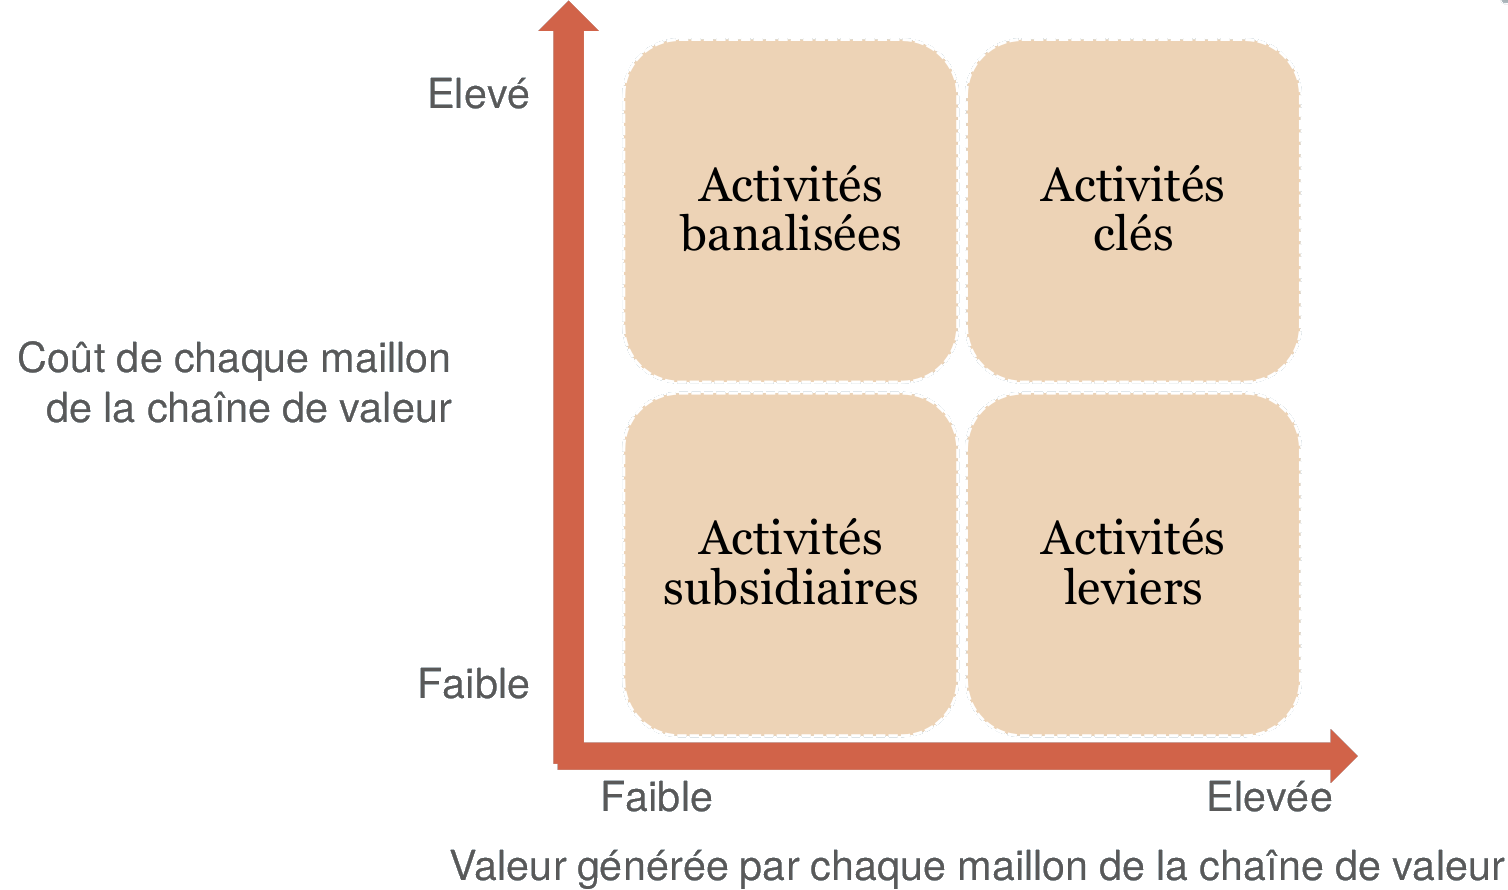
\includegraphics[width=0.7\linewidth]{benchmark_chaine_valeur.png}
\end{center}

\bigskip

C'est en analysant les activités qu'on peut trouver les activités qui
sont réellement déterminantes pour la création de valeur (appelées
parfois \og{}gisement de valeur\fg{}) et décider
d'intégrer vers l'amont ou vers l'aval si nécessaire. 

\section{Les choix stratégiques}

Les choix stratégiques se divisent majoritairement en 3 parties :

\begin{description}
    \item[Stratégies concurrentielles] : positionnenement de ses
        activités
    \item[Orientations stratégiques] : positionnement de l'organisation
    \item[Modalités de développement] : choix des acquisitions ou des
        coopérations
\end{description}

\section{La segmentation stratégique}

Soit une entreprise est mono-activité et elle forme un ensemble
homogène, alors on ne considère pas de segmentation stratégique. Soit
elle est multi-activités et elle est composée de sous-ensembles (DAS)
qui auront chacun une stratégie : c'est la \textbf{segmentation
stratégique}.

\begin{center}
    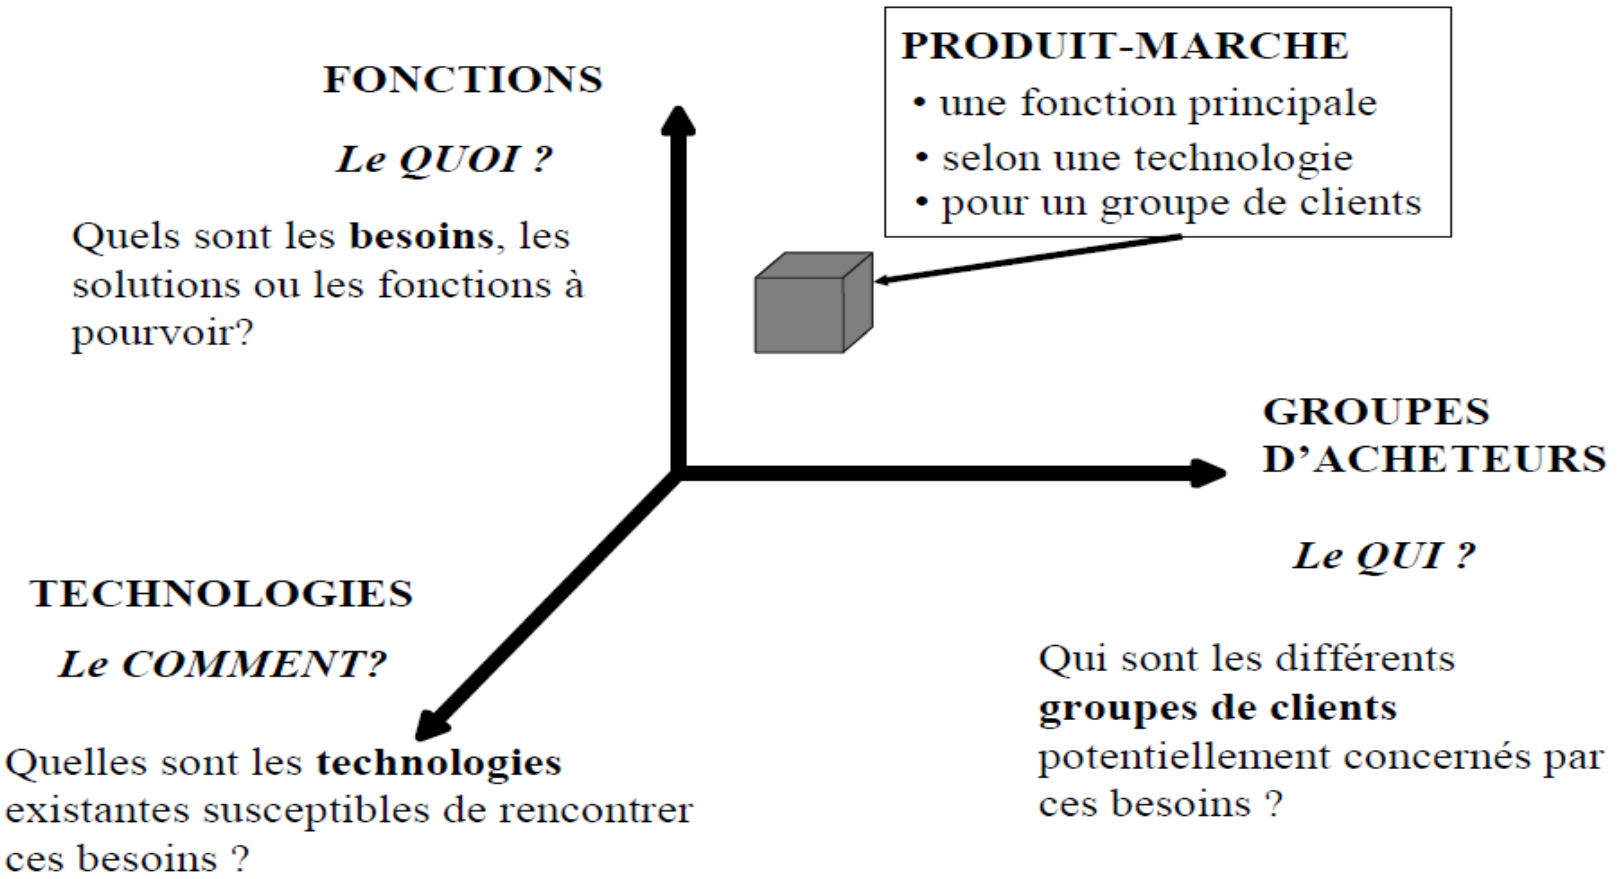
\includegraphics[width=\linewidth]{segmentation_strategique}
\end{center}

\subsection{Comment segmenter ?}

En fonction des :

\begin{itemize}
    \item besoins satisfaits
    \item technologies utilisées
    \item clients servis
\end{itemize}

Si une ou plusieurs sous-sections répondent aux mêmes caractéristiques,
on peut en faire un seul et même DAS. On pourra ainsi profiter des
\textbf{effets de synergie}. \newline

Ceci rappelle quelque chose d'important : la segmentation stratégique et
la segmentation marketing sont deux choses différentes. En effet, la
segmentation marketing ne prend en compte que les clients
servis.\newline 

\section{Les stratégies concurrentielles}

Les stratégies concurrentiels (ou \textit{génériques}) sont des
positionnements qui permettent d'obtenir un avantage concurrentiel au
niveau d'un domaine d'activité stratégique. \newline

\begin{center}
    \fbox{\begin{minipage}{0.5\linewidth}

\[
    \Delta \frac{\textrm{Valeur créée pour ses clients}}{\textrm{Coûts
    engagés par son das}} > 0
\]
\end{minipage}}

\fbox{\begin{minipage}{0.95\linewidth}

\[
    \Delta \frac{\textrm{Valeur créée pour ses clients}}{\textrm{Coûts
    engagés par son DAS}} > \Delta \frac{\textrm{Valeur créée pour les clients
    concurrents}}{\textrm{Coûts engagés par les concurrents}}
\]
\end{minipage}}
\end{center}

Autrement dit, si on veut vérifier qu'on a bien un avantage
concurrentiel il faut qu'à tout moment le rapport entre la valeur crée
et les coûts doit être supérieure de \textbf{manière permanente}.

\subsection{Les types de stratégies}

Si on veut viser la masse avec des prix bas, on a une stratégie de
\textbf{domination par les coûts}. \newline

Si on veut viser la masse mais avec des prix moyens ou élevés, on
développe une stratégie de \textbf{différentiation}. L'idée va être de
proposer des offres dont la valeur \textit{perçue} est différente. On
peut faire de la différenciation vers le haut (sophistication, proposer
mieux et beaucoup plus cher) ou de la
différenciation vers le bas (épuration, proposer moins bien un peu moins
cher). \newline 

Si on veut viser une cible étroite, on adopte une stratégie de
\textbf{focalisation}. L'idée va être d'attaquer une \textit{niche} avec
une offre fortement différencie pour un marché très spécifique (luxe,
spécialisation ou au contraire offre minimaliste).

\subsection{L'horloge stratégique de Bowman}

Ce modèle permet de placer la stratégie des entreprises au sein d'un
marché. On définit une offre de référence (typiquement, on prend du milieu de gamme à
prix moyen) \newline

\begin{center}
    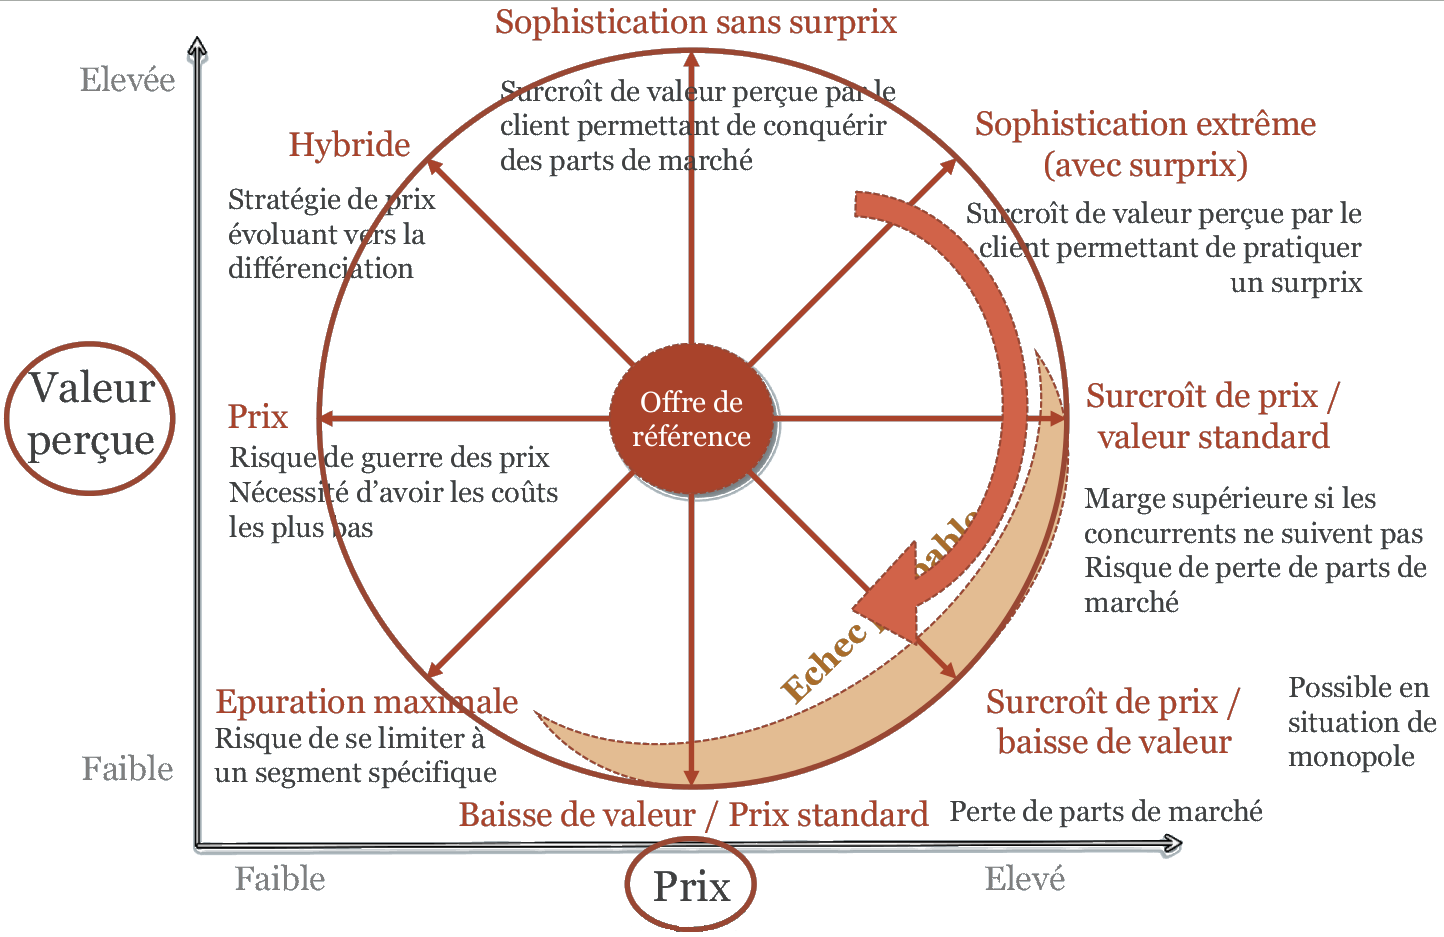
\includegraphics[width=\linewidth]{horloge_bowman.png}
\end{center}

\begin{center}
    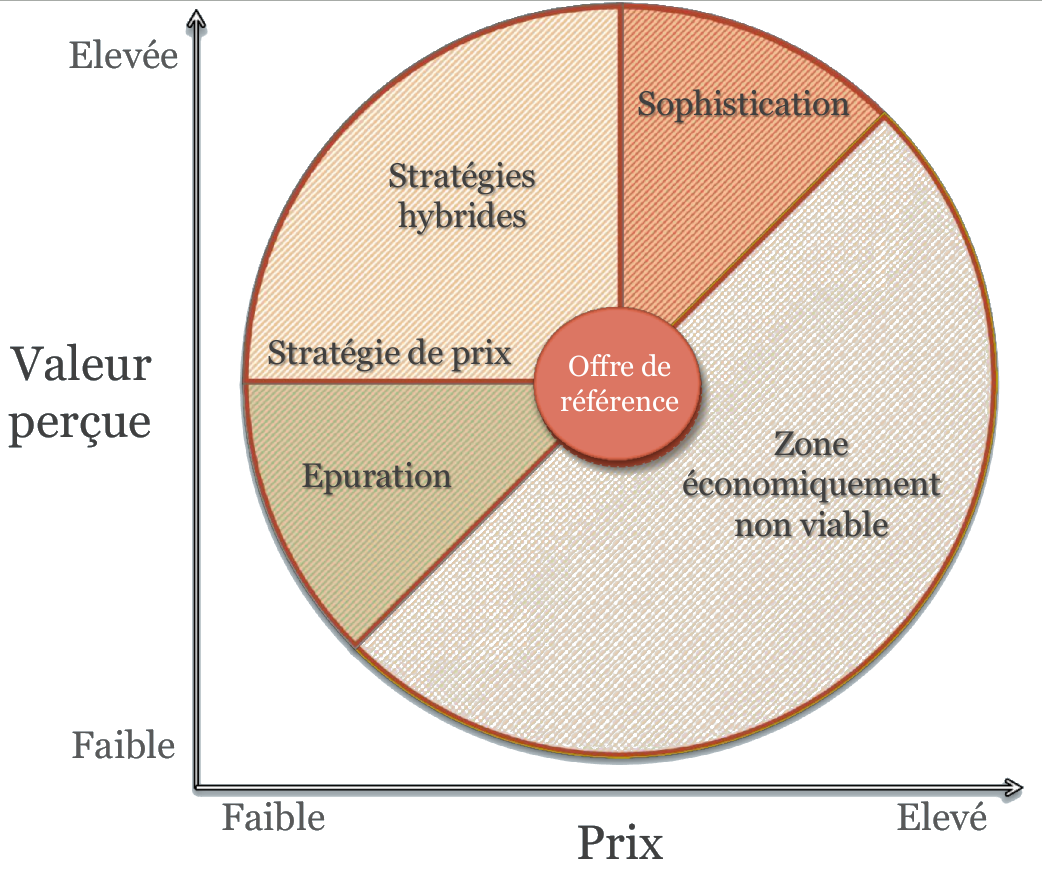
\includegraphics[width=0.8\linewidth]{horloge_bowman2.png}
\end{center}

L'horloge de Bowman est dynamique et implique des déplacements pour 2
raisons :

\begin{enumerate}
    \item Une entreprise peut changer son prix, améliorer ou déteriorer
        la valeur perçue par son produit
    \item L'offre de référence peut changer, si la moyenne du marché se
        met à offrir bien mieux pour le même prix et que vous ne suivez
        pas, vous risquez de tomber dans une zone économiquement non
        viable.
\end{enumerate}

\subsubsection{Le verrouillage}

Le verrouillage est une technique consistant à rendre les clients
dépendants de son offre en imposant des coûts de transfert
élevés.\newline

Par exemple, les cartouches pour les imprimantes, les lames pour les
rasoirs,\ldots Si l'entreprise arrive à devenir un standard de
l'industrie, c'est une forme de verrouillage (p.e: Windows, la suite
Office, Caterpillar,\ldots).

\section{Les orientations stratégiques}

\subsection{La matrice d'Ansoff - diversification}

\begin{center}
    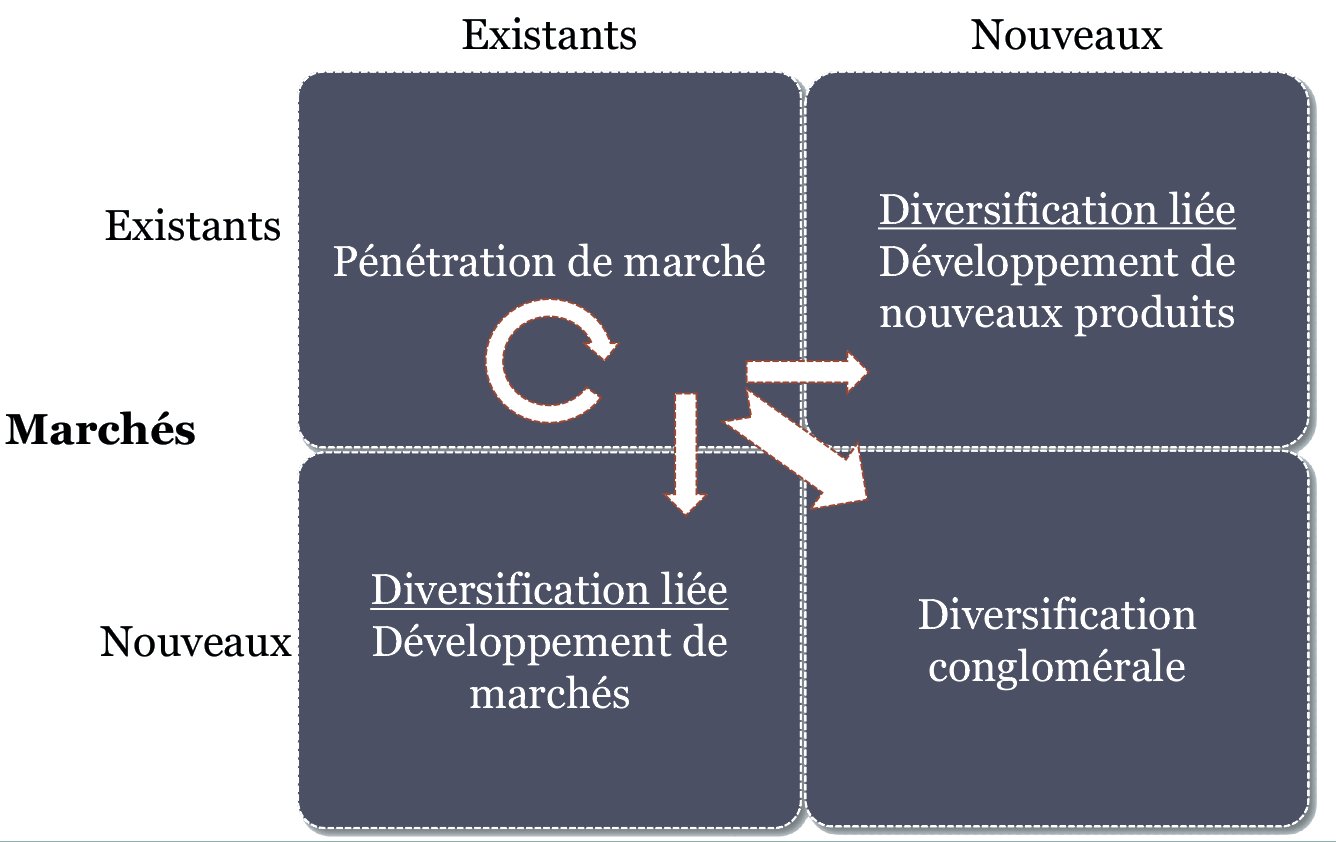
\includegraphics[width=\linewidth]{matrice_ansoff.png}
\end{center}

La \textbf{diversification} consiste à élargir la gamme de produits ou les
marchés de l'entreprise. \newline

La \textbf{diversification liée} consiste à développer des nouvelles
activités qui ont des points communs avec des activités existantes de
l'entreprise. \newline

La \textbf{diversification conglomérale} consiste à développer des
activités qui n'ont aucun point commun avec les activités
existantes.\newline

\subsection{Différentes orientations}

\begin{description}
    \item[Pénétration de marché] : augmenter les parts de marchés grâce
        à notre avantage concurrentiel (risque de guerre de prix et lois
        sur les positions dominantes)
    \item[Développement de porduits] : offrir des nouveaux produits sur
        les marchés existants
    \item[Développement de marchés] : offrir les mêmes produits sur des
        nouveaux marchés (internationalisation ou nouveaux usages du
        produit)
    \item[Diversification conglomérale] : faire autre chose, ailleurs
\end{description}

Les lois sur les positions dominantes peuvent être contrôlées par
l'indice de concentration de marché d'Herfindhal-Hirschmann.

\[
   HHI = \sum_{i=1}^{n} s_{i}^{2}
\]

L'idée est de regarder le changement du HHI avant et après le rachat
possible d'une société par une autre. Si la différence est trop grande,
alors certains organismes d'Etat peuvent interdire cette acquisition.
\newline

\subsection{Les facteurs de diversification}

Pourquoi se diversifier ?

\begin{enumerate}
    \item Faire des économies de champ (mettre ses ressources et
        compétences sur des nouveaux marchés)
    \item Par logique dominante : profiter des compétences de gestion de
        la direction générale
    \item Les marchés internes : mobilisation de ressources sur les
        marchés non matures
    \item Le pouvoir de marché : accroître son pouvoir contre les
        concurrents
    \item En réaction à un déclin
    \item Pour la répartition des risques
    \item Par ambition des dirigeants
\end{enumerate}

\subsection{Intégration - Acquisition - Fusion}

L'\textbf{intégration verticale} consiste à acheter ou fusionner (en amont ou en
aval) dans sa propre filière. \newline

L'\textbf{intégration horizontale} consiste à acheter ou fusionner des
concurrents. \newline

Au contraire, certaines entreprises font de la \textbf{désintégration
verticale}. Il arrive qu'une entreprise se rende compte que certaines
activités ne lui sont pas profitables car d'autres sont meilleures
qu'elle dans ce domaine, elle se recentre sur ses core-competences en
confiant une part de ses activités à des prestataires externes.

\end{document}
